\documentclass[12pt,onecolumn,letterpaper]{article}
\usepackage{amsmath}
\usepackage{amssymb}
\usepackage{graphicx}
\usepackage{fancyvrb}
\usepackage{cite}
%\usepackage[ampersand]{easylist}
\usepackage{listings}
\usepackage[margin=0.5in]{geometry}
\bibliographystyle{plain}
%\usepackage{marginnote}

\newcommand{\indep}{\rotatebox[origin=c]{90}{$\models$}}
\DeclareMathOperator*{\argmin}{arg\,min}
\DeclareMathOperator*{\argmax}{arg\,max}
\setlength\parindent{0.2in}

\usepackage{color}
\newcommand{\todo}[1]{{\color{red} #1}}
 
\definecolor{codegreen}{rgb}{0,0.6,0}
\definecolor{codegray}{rgb}{0.5,0.5,0.5}
\definecolor{codepurple}{rgb}{0.58,0,0.82}
\definecolor{backcolour}{rgb}{0.95,0.95,0.92}
 
\lstdefinestyle{mystyle}{
    backgroundcolor=\color{backcolour},   
    commentstyle=\color{codegreen},
    keywordstyle=\color{magenta},
    numberstyle=\tiny\color{codegray},
    stringstyle=\color{codepurple},
    basicstyle=\footnotesize,
    breakatwhitespace=false,         
    breaklines=true,                 
    captionpos=b,                    
    keepspaces=true,                 
    numbers=left,                    
    numbersep=5pt,                  
    showspaces=false,                
    showstringspaces=false,
    showtabs=false,                  
    tabsize=2
}
 
\lstset{style=mystyle}

\graphicspath{{Figures/}}

\begin{document}

%\begin{minipage}{0.5\textwidth}
%\begin{flushleft}
%    \subsection*{NAME: Tanmay Gupta}
%\end{flushleft}
%\end{minipage}
%\hfill
%\begin{minipage}{0.5\textwidth}
%\begin{flushright}
%    \subsection*{NET ID: tgupta6}
%\end{flushright}
%\end{minipage}

%\begin{minipage}{0.5\textwidth}
%\begin{flushleft}
%    \subsection*{NAME: Peter Maginnis}
%\end{flushleft}
%\end{minipage}
%\hfill
%\begin{minipage}{0.5\textwidth}
%\begin{flushright}
%    \subsection*{NET ID: maginni1}
%\end{flushright}
%\end{minipage}\begin{center}
%    \Large\textbf{IE598: Inference in Graphical Models}\\
%    \textbf{Homework 3}
%\end{center}

\title{Adaptive Crowdsourcing via EM with Prior}
\author{Peter Maginnis and Tanmay Gupta}
\maketitle

In this work, we make two primary contributions: derivation of the EM update for the shifted and rescaled beta prior and the development of an algorithm to adaptively select new edges (task assignments) for more efficient use of an edge budget (i.e. reduced probability of task labeling error for a fixed number of edges).  The algorithm exploits several observable features of a task (namely the entropy of its label probabilities, the number of workers already assigned to it, and a histogram of estimated worker abilities for its neighbors) to produce a ranking of tasks most likely to be currently mislabeled.  An additional worker (sampled uniformly) is then assigned to each of the highest ranking tasks and the graph is updated.  Rankings are produced by a random forest classifier that is given the current graph structure and prior information, and trained on ensembles of randomly generated data. 

First, we derive the EM updates for the crowdsourcing problem both without and with knowledge of the transformed beta prior.  Next we outline the adaptive algorithm used to assign edges in graph construction using the random forest classifier.  Finally, we present numerical results demonstrating the effectiveness of these techniques over a range of edge budgets.
\section{Expectation-Maximization for Crowdsourcing}
\subsection*{EM without prior}
We treat $\textbf{A}$ as our observed variables, $\textbf{t}$ as latent variables and $\textbf{p}$ as parameters. Then the joint distribution will be given as:
\begin{align*}
\mathbb{P}(\textbf{A},\textbf{t}|\textbf{p}) &= \mathbb{P}(\textbf{A}|\textbf{t},\textbf{p})\mathbb{P}(\textbf{t}|\textbf{p}) \\
&= \mathbb{P}(\textbf{A}|\textbf{t},\textbf{p})\mathbb{P}(\textbf{t}) \tag{Since true labels are independent of worker abilities} \\
&=\prod_{(i,j)\in E}\mathbb{P}(A_{ij}|t_i,p_j)\prod_{i}^{n}\mathbb{P}(t_i) \\
\end{align*}

\noindent
where,
\begin{align*}
\mathbb{P}(A_{ij}|t_i,p_j) &= p_j\mathbb{I}(A_{ij}=t_i)+(1-p_j)\mathbb{I}(A_{ij}=-t_i) \\
\mathbb{P}(t_i) &= 
\frac{3}{4}\mathbb{I}(t_i=1)+\frac{1}{4}\mathbb{I}(t_i=-1)
\end{align*}

\subsubsection*{E-Step:}
In the \textbf{E} step we find the distribution of the latent variables as a function of the observed variables and parameters estimated in the previous iteration.
\begin{align*}
\mathbb{P}(\textbf{t}|\textbf{A},\textbf{p}^{{\rm old}}) &= 
\prod_{i=1}^{n} \mathbb{P}(t_i|\textbf{A},\textbf{p}^{{\rm old}})
\end{align*}

\noindent
where,
\begin{align*}
\mathbb{P}(t_i|\textbf{A},\textbf{p}^{{\rm old}}) &=
\mathbb{P}(t_i|A_{i\partial i},p_{\partial i}^{{\rm old}}) \\
&= 
\frac{
\mathbb{P}(A_{i\partial i},t_i|p_{\partial i}^{{\rm old}})
} 	
{
\mathbb{P}(A_{i\partial i}|p_{\partial i}^{{\rm old}})
} \\
&=
\frac{
\mathbb{P}(t_i)\prod_{j\in \partial i} \mathbb{P}(A_{ij}|t_i,p_j^{{\rm old}})
}
{
\sum_{t_i} \mathbb{P}(t_i)\prod_{j\in \partial i} \mathbb{P}(A_{ij}|t_i,p_j^{{\rm old}})
} \\
&= \gamma_i(t_i)
\end{align*}
In the sequel, allowing for a slight abuse of notation, we need only refer to
\begin{align*}
  \gamma_i:=\gamma_i(1)&=\mathbb{P}(t_i=1|\textbf{A},\textbf{p}^{{\rm old}})\\
  &=\frac{\mathbb{P}(A_{i\partial i}|t_i=1,{\bf p})\mathbb{P}(t_i=1)}{\mathbb{P}(A_{i\partial i}|t_i=1,{\bf p})\mathbb{P}(t_i=1)+\mathbb{P}(A_{i\partial i}|t_i=-1,{\bf p})\mathbb{P}(t_i=-1)}\\
  &=\frac{\frac{3}{4}\prod_{j\in\partial i} p_j^{\mathbb{I}(A_{ij}=1)}(1-p_j)^{\mathbb{I}(A_{ij}=-1)}}{\frac{3}{4}\prod_{j\in\partial i} p_j^{\mathbb{I}(A_{ij}=1)}(1-p_j)^{\mathbb{I}(A_{ij}=-1)}+\frac{1}{4}\prod_{j\in\partial i} p_j^{\mathbb{I}(A_{ij}=-1)}(1-p_j)^{\mathbb{I}(A_{ij}=1)}}\\
  &=\frac{\frac{3}{4}\prod_{j\in\partial i} \left[\frac{1}{2}+\frac{2p_j-1}{2}A_{ij}\right]}{\frac{3}{4}\prod_{j\in\partial i} \left[\frac{1}{2}+\frac{2p_j-1}{2}A_{ij}\right]+\frac{1}{4}\prod_{j\in\partial i} \left[\frac{1}{2}-\frac{2p_j-1}{2}A_{ij}\right]}
\end{align*}
\subsubsection*{M-Step:}
In this we approximate the log likelihood of the observed data using the expected log likelihood of the observed and latent variables together where the expectation is with respect to the distribution of the latent variables computed in the \textbf{E} step
\begin{align*}
Q(\textbf{p}|\textbf{p}^{{\rm old}}) &= 
\mathbb{E}_{
{\bf \gamma}
}
\left[
\log{
\mathbb{P}(\textbf{A},\textbf{t}|\textbf{p})
}
\right] \\
&=
\mathbb{E}_{
\textbf{t}|\textbf{A},\textbf{p}^{{\rm old}}
}
\left[
\log{
\mathbb{P}(\textbf{A},\textbf{t}|\textbf{p})
}
\right] \\
&=
\sum_{\textbf{t}\in \{-1,1\}^n} 
\mathbb{P}(\textbf{t}|\textbf{A},\textbf{p}^{{\rm old}})
\log{
\mathbb{P}(\textbf{A},\textbf{t}|\textbf{p})
} \\
&= 
\sum_{\textbf{t}\in \{-1,1\}^n}
\left[
\left(
\prod_{i=1}^{n} \mathbb{P}(t_i|\textbf{A},\textbf{p}^{{\rm old}})
\right)
\sum_{i=1}^{n}
\left(
\log{\mathbb{P}(t_i|\textbf{p})} +
\sum_{j\in \partial i} 
\log \mathbb{P}(A_{ij}|t_i,p_j) 
\right)
\right] \\
&=
\sum_{i=1}^{n}
\sum_{t_i} \gamma_i(t_i) 
\left[
\log{\mathbb{P}(t_i|\textbf{p})} +
\sum_{j\in \partial i} 
\log \mathbb{P}(A_{ij}|t_i,p_j) 
\right] \\
&=
\sum_{i=1}^{n}
\Bigg\{\gamma_i 
\left[
\log{\mathbb{P}(t_i=1)} +
\sum_{j\in \partial i} 
\log \mathbb{P}(A_{ij}|t_i=1,p_j) 
\right]\\
&\qquad+(1-\gamma_i)
\left[
\log{\mathbb{P}(t_i=-1)} +
\sum_{j\in \partial i} 
\log \mathbb{P}(A_{ij}|t_i=-1,p_j) 
\right]
\Bigg\}
\end{align*}

\noindent
Now to maximize $Q(\textbf{p}|\textbf{p}^{{\rm old}})$ with respect to $\textbf{p}$ we set the derivatives to zero.
\begin{align*}
& \frac{\partial{Q}}{\partial{p_j}} = 0 \\
%\implies &
%\sum_{i\in \partial j} 
%\sum_{t_i} \gamma_i(t_i)
%\left(
%\frac{1}{p_j}\mathbb{I}(A_{ij}=t_i) -
%\frac{1}{1-p_j}\mathbb{I}(A_{ij}=-t_i)
%\right) 
%= 0 \\
\implies &
\sum_{i\in \partial j} 
\left[
\gamma_i
\left(
\frac{\mathbb{I}(A_{ij}=1)}{p_j} -
\frac{\mathbb{I}(A_{ij}=-1)}{1-p_j}
\right) +
\left(1-\gamma_i\right)
\left(
\frac{\mathbb{I}(A_{ij}=-1)}{p_j} -
\frac{\mathbb{I}(A_{ij}=1)}{1-p_j}
\right) 
\right]
= 0 \\
\implies &
\sum_{i\in \partial j} 
\left[
\left(
\gamma_i-p_j
\right) 
\mathbb{I}(A_{ij}=1) +
\left(
1-\gamma_i - p_j
\right) 
\mathbb{I}(A_{ij}=-1)
\right] 
= 0 \\
\implies &
p_j = 
\frac{1}{|\partial j|}
\sum_{i\in \partial j} 
\left[\gamma_i
\mathbb{I}(A_{ij}=1) +
\left(
1-\gamma_i
\right) 
\mathbb{I}(A_{ij}=-1)\right]
\end{align*}

\subsection*{EM with Beta Prior}

Instead, we seek to maximize the objective 
\begin{align*}
   Q({\bf p}|{\bf p}^{\rm old})&=\mathbb{E}_{\gamma}\left[\ln\mathbb{P}(\bf{A}|\bf{p})+\ln\mathbb{P({\bf p})}\right]\\
   &=\sum_{i=1}^n \left[\gamma_i\ln{\frac{3}{4}a_i+(1-\gamma_i)\ln\frac{1}{4}b_i}\right]+\sum_{j=1}^m\ln f\left(\frac{p_j-0.1}{0.9}\right),
\end{align*}
where 
\begin{align*}
a_i&:=\mathbb{P}(A_{i\partial i}|t_i=1,{\bf p})=\prod_{j\in\partial i} p_j^{\mathbb{I}(A_{ij}=1)}(1-p_j)^{\mathbb{I}(A_{ij}=-1)}\\
b_i&:=\mathbb{P}(A_{i\partial i}|t_i=-1,{\bf p})=\prod_{j\in\partial i} p_j^{\mathbb{I}(A_{ij}=-1)}(1-p_j)^{\mathbb{I}(A_{ij}=1)},
\end{align*}
and
\begin{equation*}
 f(z)=\frac{1}{B(\alpha,\beta)}(z)^{\alpha-1}(1-z)^{\beta-1}
\end{equation*}
We take the gradient
\begin{align*}
   \frac{\partial{Q}}{\partial{p_j}}&=\sum_{i\in\partial j}\left\{\gamma_i\left[\frac{\mathbb{I}(A_{ij}=1)}{p_j}-\frac{\mathbb{I}(A_{ij}=-1)}{1-p_j}\right]+(1-\gamma_i)\left[\frac{\mathbb{I}(A_{ij}=-1)}{p_j}-\frac{\mathbb{I}(A_{ij}=1)}{1-p_j}\right]\right\}+\frac{\alpha-1}{p_j-0.1}-\frac{\beta-1}{1-p_j}\\
   &=\sum_{i\in\partial j}\left\{\frac{\gamma_i\mathbb{I}(A_{ij}=1)+(1-\gamma_i)(\mathbb{I}(A_{ij}=-1))}{p_j}-\frac{(1-\gamma_i)\mathbb{I}(A_{ij}=1)+\gamma_i(\mathbb{I}(A_{ij}=-1))}{1-p_j}\right\}+\frac{\alpha-1}{p_j-0.1}-\frac{\beta-1}{1-p_j}\\
   &=\sum_{i\in\partial j}\left\{\frac{\gamma_iA_{ij}-A_{ij}+1}{p_j}-\frac{A_{ij}-\gamma_iA_{ij}+1}{1-p_j}\right\}+\frac{\alpha-1}{p_j-0.1}-\frac{\beta-1}{1-p_j}.
\end{align*}
We then solve for the critical point
\begin{align*}
\frac{\partial{Q}}{\partial{p_j}}=0
\end{align*}
which implies
\begin{align*}
  0=(p_j-0.1)\sum_{i\in\partial j}\left\{\gamma_i\mathbb{I}(A_{ij}=1)+(1-\gamma_i)\mathbb{I}(A_{ij}=-1)-p_j\right\}+(\alpha-1)p_j(1-p_j)-(\beta-1)p_j(p_j-0.1).
\end{align*}
Define
\begin{equation*}
  \lambda_j:=\frac{1}{|\partial j|}\sum_{i\in\partial j}\left[\gamma_i\mathbb{I}(A_{ij}=1)+(1-\gamma_i)\mathbb{I}(A_{ij}=-1)\right].
\end{equation*}
Then, we may more compactly write the quadratic equation
\begin{equation*}
  0=(p_j-0.1)|\partial j|(\lambda_j-p_j)+(\alpha-1)p_j(1-p_j)-(\beta-1)p_j(p_j-0.1).
\end{equation*}
Numerical results indicate that the smaller root lies outside the support, $[0.1,1]$, of the worker ability distribution, and the larger root is always taken for the EM update. 

Note that if, instead, we model $p_j$ as $\operatorname{Beta}(\alpha,\beta)$, then the above analysis recovers the update found in~\cite{LiPeIh2012,RaYuZhVaFlBoMo2010}. Specifically, the critical equation becomes
\begin{align*}
  0&=|\partial j|(\lambda_j-p_j)+(\alpha-1)(1-p_j)-(\beta-1)p_j\\
  &\implies \lambda_j|\partial j|+\alpha-1=(|\partial j|+\alpha+\beta-2)p_j\\
  &\implies p_j=\frac{\sum_{i\in\partial j}\left[\gamma_i\mathbb{I}(A_{ij}=1)+(1-\gamma_i)\mathbb{I}(A_{ij}=-1)\right]+\alpha-1}{|\partial j|+\alpha+\beta-2}
\end{align*}
\section{Adaptive Graph Construction}
We adapt to the current state of the EM estimate and graph by training a random forest classifier to estimate which label assignments are most likely incorrect.  Given the current graph, the algorithm for adaptive edge assignment proceeds as follows.  At iteration $\ell$, we are given a current graph $G^{(\ell)}$ and an EM estimate $(\gamma^{(\ell)}, \hat{\bf p}^{(\ell)})$. The current graph $G^{(\ell)}$ is passed to a random forest generation algorithm that has access to the $\bf{t}$ and $\bf{p}$ prior distributions.  The random forest generator then runs EM on ensembles of i.i.d. randomly generated instances of $({\bf A^{(\ell)},t^{(\ell)},p^{(\ell)}})_e$ to produce task label probabilies ${\hat{\bf{\gamma}}^{(\ell)}}_e$ and worker ability maximum likelihood estimates $\hat{\bf p}^{(\ell)}_e$ and trains a random forest classifier using entropy of label probability estimates $h(\hat\gamma^{(\ell)}_e)$, number of workers assigned to a task $|\partial i^{(\ell)}|$, and a histogram of $\{\hat{p}^{(\ell)}_{\partial i}\}$ as features and incorrectness of task assignments as the true labels.  The resulting random forest classifier is then returned to the main algorithm, which uses the random forest and EM estimates of the current graph to rank the actual tasks by likelihood of mislabeling.  The $K$ highest risk tasks $\{i_k\}_{k=1}^K$ are then assigned one new worker chosen uniformly from the population of workers who are not already assigned to that task.  These edges are then added to $G^{(\ell)}$ to produce $G^{(\ell+1)}$.
\subsection{Random Forest}
Random forest~\cite{Bre2001} is an ensemble machine learning algorithm that has wide applicability in classification and regression tasks. The basic unit of a random forest is a decision tree. Each node in the tree represents a binary decision on a feature and every path from the root to a leaf represents a logical conjunction of the binary decisions encountered along the path. Learning a decision tree from data $\mathcal{D}=\{(\textbf{x}_i,l_i)|i=1,\cdots,M\}$ comprising of $M$ $($feature, label$)$ pairs involves choosing a feature and a threshold that forms the splitting criterion for each node and assigning each $\textbf{x}_i$ to one of the leaves, $L_i$ in the tree where $L_i \in \{1,\cdots, N\}$ if there are $N$ leaves in the tree. During inference a new feature vector $\textbf{v}$ follows a path from the root to some leaf $L$ in the tree and gets a class posterior distribution given by
\begin{equation*}
P(l|\textbf{v}) = \frac{\sum_{i=1}^{M}\mathbb{I}(L_i=L)\mathbb{I}(l_i=l)}
{\sum_{i=1}^{M}\mathbb{I}(L_i=L)}.
\end{equation*}

The splitting criterion is chosen using some notion of information gain such as decrease in entropy after splitting. Let left$(i)$ and right$(i)$ denote the left and right children of node $i$ and $p_i(l)$ be the fraction of training data points that reached node $i$ which had label $l$. Then the information gain for a particular splitting criterion is evaluated as follows:
\begin{equation*}
\Delta = \sum_{j=1}^{C}p_i(l_j)\log{p_i(l_j)} - \left[\sum_{j=1}^{C}p_{\mathrm{left}(i)}(l_j)\log{p_{\mathrm{left}(i)}(l_j)} - 
\sum_{j=1}^{C}p_{\mathrm{right}(i)}(l_j)\log p_{\mathrm{right}(i)}(l_j)\right] 
\end{equation*}
The feature and threshold used for splitting at a node is the one that maximizes $\Delta$. 

Random forest is simply a way to reduce over-fitting in a decision tree by using ensemble of decision trees where each tree is trained on a subset of randomly sampled training data. Inference on a random forest is done by passing $\textbf{v}$ through each tree and then averaging their predictions. So the final posterior class probabilities are 
\begin{equation*}
P(l|\textbf{v}) = \frac{1}{T} \sum_{t=1}^{T} P_t(l|\textbf{v})
\end{equation*}
where $T$ is the number of trees and $P_t$ is probability obtained from the $t^{th}$ tree.

\begin{figure}
\centering
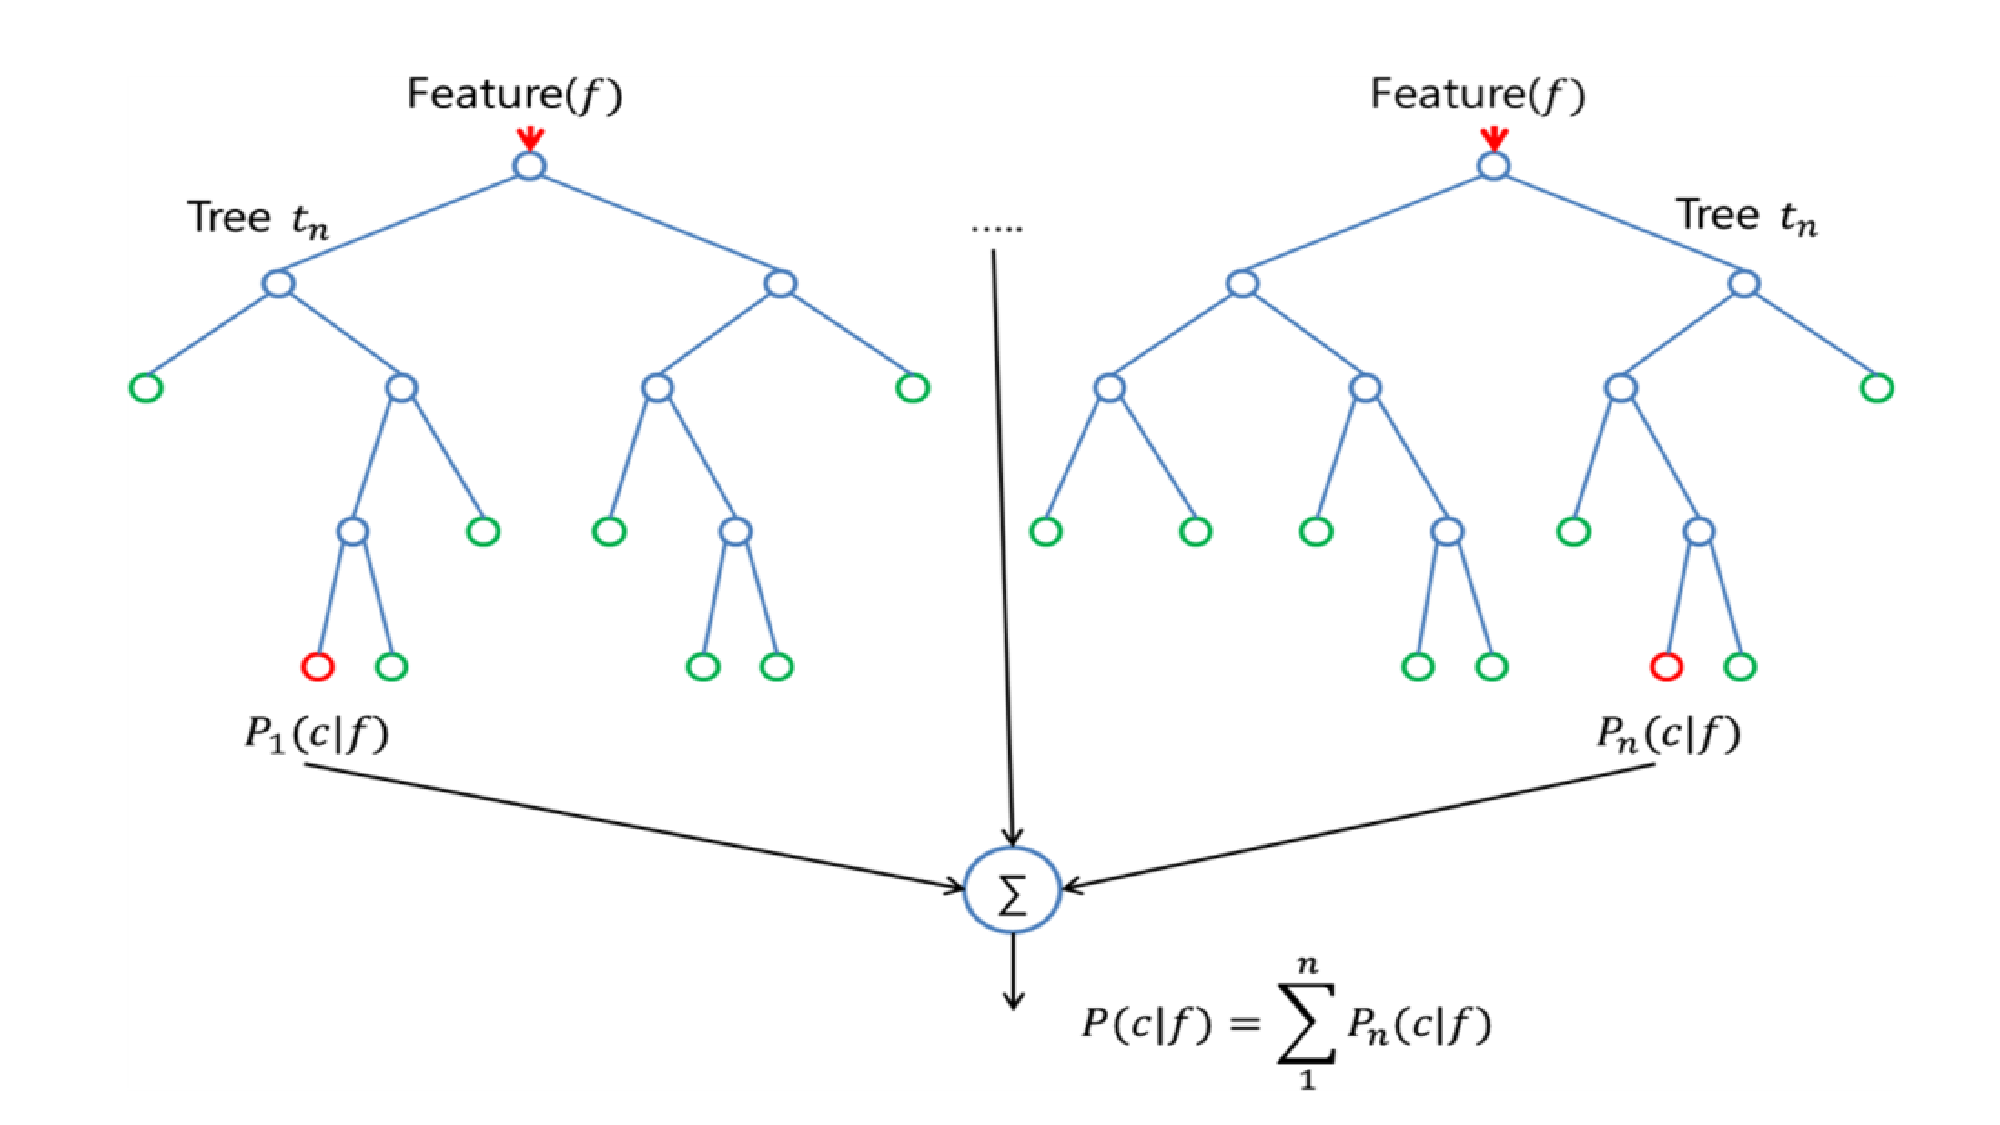
\includegraphics[width=5in]{Random_Forest.pdf}
\caption{Illustration of the random forest technique, whereby an ensemble of decision trees are combined to produce an estimate of the probability of a correct response.  Image from~\cite{KiKa2013}}
\label{fig:rf}
\end{figure} 

\section{Numerical Results}
To examine the performance of our two contributions over a range of edge budget values, we consider a bipartite graph initialization $G^{(0)}$ that assigns one worker to every task and at least one task to each of $m<n$ workers, using the fewest edges possible (2000).  As a baseline for comparison, we consider a technique where at each step $\ell$, we add edges by sampling uniformly from the tasks $i\in[n]$ and then uniformly selecting a worker not already assigned to that task, $j\in[m]\setminus\partial i$. We then proceed by adding edges (either randomly or adaptively) and computing the EM estimates periodically. The results of averaging 100 such experiments are show in Figure~\ref{fig:mean_err_100_workers}

\begin{figure}
\centering
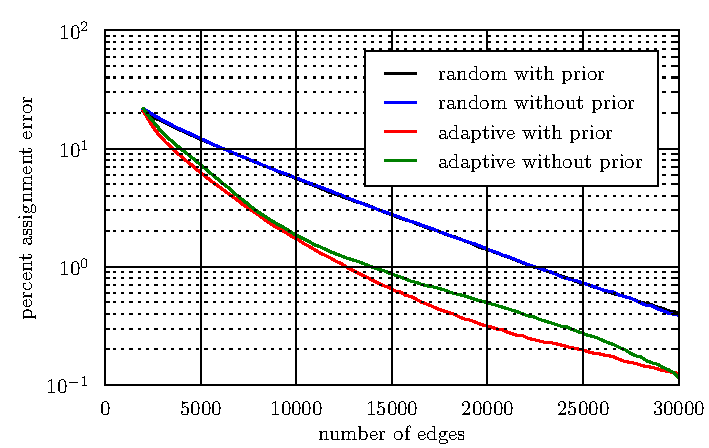
\includegraphics[width=5in]{py_mean_perc_err_100_workers.pdf}
\caption{Mean percent classification error for the 4 modes of estimation: random graph construction both with and without transformed beta prior and adaptive graph construction using EM with and without the transformed beta prior.  Note that in the random graph generation cases, the results of EM both with and without prior are almost identical.  However, when graph construction is done adaptively, and thus depends on the output of EM, we see a marked improvement by including worker ability prior data.}
\label{fig:mean_err_100_workers}
\end{figure} 



\begin{thebibliography}{99}
\bibitem{LiPeIh2012} Q. Liu, J. Peng, and A. T. Ihler. ``Variational Inference for Crowdsourcing''. {\it Advances in Neural Information Processing Systems}, 2012. 
\bibitem{RaYuZhVaFlBoMo2010} V. C. Raykar, S. Yu, L. H. Zhao, G. H. Valadez, C. Florin, L. Bogoni, and L. Moy. ``Learning from crowds''. {\it The Journal of Machine Learning Research}, 11:1297-1322, 2010.
\bibitem{Bre2001} L. Breiman. ``Random Forests''. {\it Machine Learning}, vol. 45(1):5-32, 2001.
\bibitem{KiKa2013} O. Kim and D. J. Kang. ``Fire detection system using random forest classification for image sequences of complex background''. {\it Optical Engineering}, 52(6), 067202, 2013. 
%\bibitem{RaPeCaGi2005} M. Rathinam, L. R. Petzold, Y. Cao, and D. T. Gillespie, ``Consistency and stability of tau-leaping schemes for chemical reaction systems''. {\it Multiscale Modeling and Simulation}, vol. 4(3):867�895, 2005.
\end{thebibliography}
\end{document}
